% $Header$

\documentclass{beamer}

% This file is a solution template for:

% - Talk at a conference/colloquium.
% - Talk length is about 20min.
% - Style is ornate.



% Copyright 2004 by Till Tantau <tantau@users.sourceforge.net>.
%
% In principle, this file can be redistributed and/or modified under
% the terms of the GNU Public License, version 2.
%
% However, this file is supposed to be a template to be modified
% for your own needs. For this reason, if you use this file as a
% template and not specifically distribute it as part of a another
% package/program, I grant the extra permission to freely copy and
% modify this file as you see fit and even to delete this copyright
% notice. 


\mode<presentation>
{
  \usetheme{Warsaw}
  % or ...

  \setbeamercovered{transparent}
  % or whatever (possibly just delete it)
}


\usepackage[english]{babel}
% or whatever

\usepackage[utf8]{inputenc}
% or whatever

\usepackage{tikz}
\usetikzlibrary{arrows, shapes, snakes}

\usepackage{times}
\usepackage[T1]{fontenc}
% Or whatever. Note that the encoding and the font should match. If T1
% does not look nice, try deleting the line with the fontenc.

%\newtheorem{definition}{Definition}

\title% (optional, use only with long paper titles)
{Consensus and replication}

\subtitle
{From impossibility to production}

\author[Alexander Kharitonov]{Alexander Kharitonov \\ \texttt{skywalker@yandex-team.ru}}
\date{Yandex science seminar, 22 Mar 2012}

%\author[Author, Another] % (optional, use only with lots of authors)
%{F.~Author\inst{1} \and S.~Another\inst{2}}
% - Give the names in the same order as the appear in the paper.
% - Use the \inst{?} command only if the authors have different
%   affiliation.
%\institute[Yandex]
%{
%    Yandex LLC
%}

%\institute[Universities of Somewhere and Elsewhere] % (optional, but mostly needed)
%{
%  \inst{1}%
%  Department of Computer Science\\
%  University of Somewhere
%  \and
%  \inst{2}%
%  Department of Theoretical Philosophy\\
%  University of Elsewhere}
% - Use the \inst command only if there are several affiliations.
% - Keep it simple, no one is interested in your street address.

%\date[CFP 2003] % (optional, should be abbreviation of conference name)
%{Conference on Fabulous Presentations, 2003}
% - Either use conference name or its abbreviation.
% - Not really informative to the audience, more for people (including
%   yourself) who are reading the slides online

\subject{Distributed systems}
% This is only inserted into the PDF information catalog. Can be left
% out. 



% If you have a file called "university-logo-filename.xxx", where xxx
% is a graphic format that can be processed by latex or pdflatex,
% resp., then you can add a logo as follows:

% \pgfdeclareimage[height=0.5cm]{university-logo}{university-logo-filename}
% \logo{\pgfuseimage{university-logo}}


% If you wish to uncover everything in a step-wise fashion, uncomment
% the following command: 

%\beamerdefaultoverlayspecification{<+->}


\begin{document}

\begin{frame}
  \titlepage
\end{frame}

\begin{frame}{Outline}
  \tableofcontents
  % You might wish to add the option [pausesections]
\end{frame}


% Structuring a talk is a difficult task and the following structure
% may not be suitable. Here are some rules that apply for this
% solution: 

% - Exactly two or three sections (other than the summary).
% - At *most* three subsections per section.
% - Talk about 30s to 2min per frame. So there should be between about
%   15 and 30 frames, all told.

% - A conference audience is likely to know very little of what you
%   are going to talk about. So *simplify*!
% - In a 20min talk, getting the main ideas across is hard
%   enough. Leave out details, even if it means being less precise than
%   you think necessary.
% - If you omit details that are vital to the proof/implementation,
%   just say so once. Everybody will be happy with that.

\section{Motivation}
\subsection{Example: leader election}

\begin{frame}
  Consider a classic semi-synchronous master-slave replication scheme with quorum writes.
  \begin{figure}[!h]
  \centering
  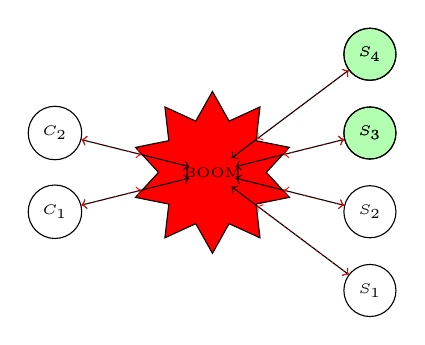
\begin{tikzpicture}
    \tikzstyle{every node} = [draw]
    \node (c1) [circle] at (0, 1) {\tiny $C_1$};
    \node (c2) [circle] at (0, 2) {\tiny $C_2$};
    \invisible<2>{\node (m)  [circle, fill=green!30] at (2, 1.5) {\tiny $M$};}
    \invisible<1>{\node (fm) [star, star points=10, fill=red] at (2, 1.5) {\tiny BOOM};}
    \node (s1) [circle] at (4, 0) {\tiny $S_1$};
    \node (s2) [circle] at (4, 1) {\tiny $S_2$};
    \visible<1> {
      \node (s3) [circle, fill=green!30] at (4, 2) {\tiny $S_3$};
      \node (s4) [circle, fill=green!30] at (4, 3) {\tiny $S_4$};
    }
    \visible<2> {
      \node (fs3) [circle] at (4, 2) {\tiny $S_3$};
      \node (fs4) [circle] at (4, 3) {\tiny $S_4$};
    }
    \invisible<2>{
      \foreach \from/\to in {c1/m, c2/m}
        \draw [<->] (\from) -- (\to);
      \foreach \from/\to in {m/s1, m/s2, m/s3, m/s4}
        \draw [<->] (\from) -- (\to);
    }
    \invisible<1>{
      \foreach \from/\to in {c1/fm, c2/fm}
        \draw [red, dotted, <->] (\from) -- (\to);
      \foreach \from/\to in {fm/s1, fm/s2, fm/s3, fm/s4}
        \draw [red, dotted, <->] (\from) -- (\to);
    }
  \end{tikzpicture}
  \end{figure}
  \visible<2>{ As we all know, manual master failover sucks. }
\end{frame}

\begin{frame}{Master election}
  \begin{itemize}
    \item  To maintain data consistency in this setting, the master election protocol \alert{must} provide the following guarantees:
      \begin{itemize}
        \item Only a single master is chosen.
        \item A participant never learns that a process $M$ is chosen to be master unless it is actually chosen.
      \end{itemize}
    \item It also makes sense to require that only an active process can be chosen (e.g. not to elect a dead replica that takes no part in the protocol).
    \item The protocol must also be fault-tolerant in some sense (remember the BOOM?).
    \item This protocol is essentially \alert{consensus} on the identity of the master.
  \end{itemize}
\end{frame}

\section{Consensus}
\subsection{On the problem and the model}
\begin{frame}{Consensus}
  \begin{itemize}
    \item Consider a collection of processes that can propose values. A \alert{consensus} algorithm ensures that a single value among the proposed ones is chosen and the processes are then able to learn the chosen value.
    \item The \alert{safety} properties of consensus are:
      \begin{itemize}
        \item Only a value that has been proposed has been chosen.
        \item Only a single value is chosen.
        \item A process never learns that a value has been chosen unless it actually has been.
      \end{itemize}
    \item The \alert{liveness} property is that if enough processes stay alive, then eventually a value is chosen and all nonfaulty processes eventually learn it.
  \end{itemize}
\end{frame}

\begin{frame}{Process roles}
  \begin{itemize}
    \item Proposers propose values.
    \item Acceptors accept proposals and determine the consensus value.
    \item Learners learn the chosen value.
  \end{itemize}
\end{frame}

\begin{frame}{A few words on the model}
  We assume the \alert{asynchronous} model with \alert{non-Byzantine} faults. It means that:
  \begin{itemize}
    \item Processes operate at arbitrary speeds, have no shared clocks and no bound on clock drift. They may fail by stopping and restart afterwards. Each process has stable storage which survives failures.
    \item Processes communicate by sending messages. Messages can take arbitrarily long to be delivered, can be duplicated, reordered and lost, but \alert{cannot be corrupted}.
  \end{itemize}
\end{frame}

\subsection{Building a safe and resilient consensus algorithm}
\begin{frame}{So let's try to build a consensus algorithm!}
  A na\"ive algorithm would use a single distinguished acceptor which chooses the first proposal it receives. It is safe, but it does not tolerate the failure of that single acceptor.
  \begin{figure}[!h]
  \centering
  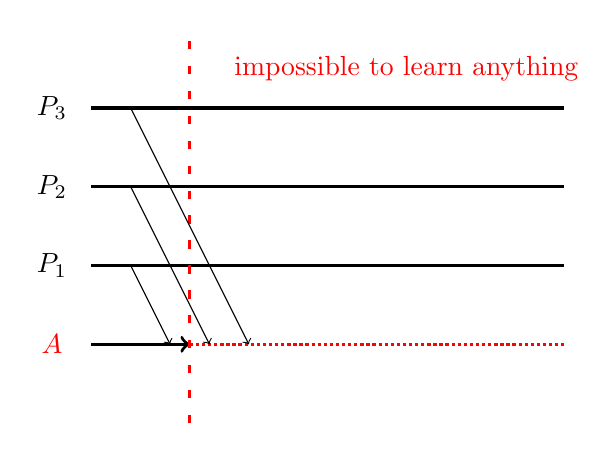
\begin{tikzpicture}
%    \tikzstyle{every node} = [draw]
    \foreach \n in {1, 2, 3} {
      \node at (-0.5, \n) {$P_\n$};
      \draw [very thick] (0, \n) -- (6, \n);
    }
    \node [red] at (-0.5, 0) {$A$};
    \node [red] at (4, 3.5) {impossible to learn anything};
    \draw [very thick, ->] (0, 0) -- (1.25, 0);
    \draw [densely dotted, very thick, red] (1.25, 0) -- (6, 0);
    \draw [loosely dashed, very thick, red] (1.25, -1) -- (1.25, 4);
    \draw [thin, ->] (0.5, 3) -- (2, 0);
    \draw [thin, ->] (0.5, 2) -- (1.5, 0);
    \draw [thin, ->] (0.5, 1) -- (1, 0);
  \end{tikzpicture}
  \end{figure}
\end{frame}

\newtheorem{invariant}[theorem]{Invariant}

\begin{frame}{Okay, let's have many acceptors!}
  \begin{itemize}
    \item Let's say that a value has been chosen when a large enough set of acceptors accepted it.
    \item Large enough -- e.g. a majority.
    \item If an acceptor can accept \alert{at most one value}, then safety is guaranteed, because any two majorities have an element in common!
    \item Without failures and message loss, want to choose a value if there is only \alert{one} proposer and it proposes \alert{one} value. This suggests the following invariant:
  \end{itemize}
  \begin{invariant}[P1]
    An acceptor must accept the first value it receives.
  \end{invariant}
\end{frame}

\begin{frame}{Just P1 and the majority rule aren't good enough}
  \begin{figure}[!h]
  \centering
  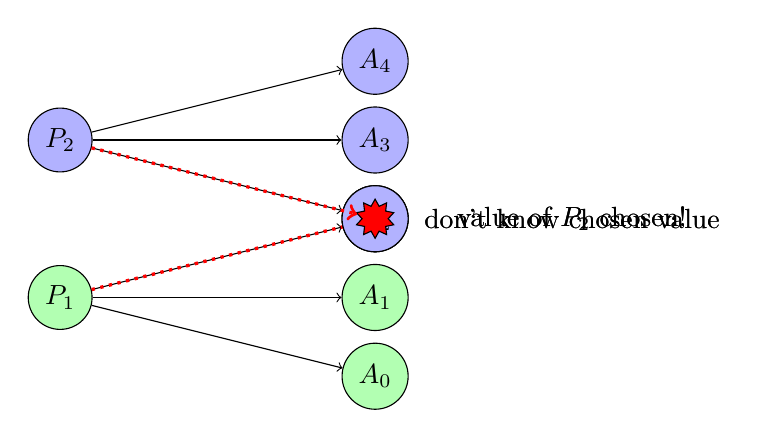
\begin{tikzpicture}
    \tikzstyle{every node} = [shape=circle]
    \node (p1) [draw, fill=green!30] at (0, 1) {$P_1$};
    \node (p2) [draw, fill=blue!30] at (0, 3) {$P_2$};
    \foreach \n in {0, 1} {
      \node (a\n) [draw, fill=green!30] at (4, \n) {$A_\n$};
      \draw [->] (p1) -- (a\n);
    }
    \foreach \n in {3, 4} {
      \node (a\n) [draw, fill=blue!30] at (4, \n) {$A_\n$};
      \draw [->] (p2) -- (a\n);
    }
    \visible<2>{
        \node (A) [draw, fill=green!30] at (4, 2) {$A_2$};
        \node at (6.5, 2) {value of $P_1$ chosen!};
        \draw [->] (p1) -- (A);
    }
    \visible<3>{
        \node (A) [draw, star, star points=10, fill=red] at (4, 2) {};
        \node at (6.5, 2) {don't know chosen value};
        \draw [dotted, very thick, ->, red] (p1) -- (A);
    }
    \visible<1,4>{
        \node (A) [draw] at (4, 2) {$A_2$};
    }
    \visible<5>{
        \node (A) [draw, fill=blue!30] at (4, 2) {$A_2$};
        \node at (6.5, 2) {value of $P_2$ chosen!};
        \draw [->] (p2) -- (A);
    }
    \visible<6>{
        \node (A) [draw, star, star points=10, fill=red] at (4, 2) {};
        \node at (6.5, 2) {don't know chosen value};
        \draw [dotted, very thick, ->, red] (p2) -- (A);
    }

  \end{tikzpicture}
  \end{figure}
\end{frame}

\begin{frame}{Multiple proposals}
  To counter this deadlock, we must allow the acceptors to accept more than one proposal.
  \begin{itemize}
    \item A proposal is a pair $(n, v)$ where $n \in \mathbb{N}$ and $v$ is a proposed value.
    \item Proposal numbers \alert{must be unique}. That means
    \begin{invariant}[P3]
      A value of the proposal is uniquely determined by its number.
    \end{invariant}
    
    {\small E.g. with $k$ proposers, the $i$-th proposer could generate proposal numbers from $\{ i + nk \mid n \in \mathbb{N} \}$.}
    \item A value is chosen when a \alert{single proposal with that value} is accepted by a majority of acceptors.
  \end{itemize}
\end{frame}

\begin{frame}{Consistency with multiple proposals}
  We must allow multiple proposals to be chosen to avoid the aforementioned deadlock, but how do we guarantee consistency?
  \begin{invariant}[P2]
    If a proposal with value $v$ is chosen, then every higher-numbered proposal that is chosen has value $v$.
  \end{invariant}
  \begin{itemize}
    \item Consistency now follows from the fact that $\mathbb{N}$ is totally ordered.
    \item How do we enforce $P2$ though?
  \end{itemize}
\end{frame}

\begin{frame}{Consistency of multiple proposals}
  \begin{invariant}[$P2^a$]
    If a proposal with value $v$ is chosen, then every higher-numbered proposal accepted by \alert{any} acceptor has value $v$.
  \end{invariant}
\end{frame}

\begin{frame}{$P2^a$ doesn't play well with $P1$}
  \begin{figure}[!h]
  \centering
  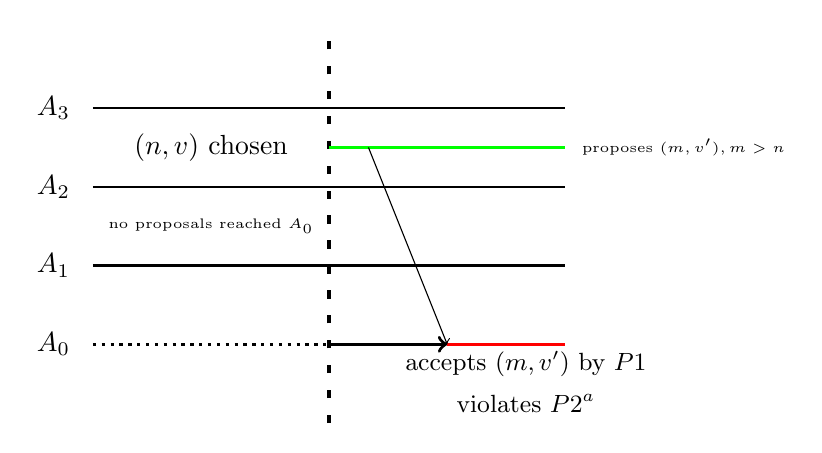
\begin{tikzpicture}
%    \tikzstyle{every node} = [draw]
    \foreach \n in {1, 2, 3} {
      \node at (-0.5, \n) {$A_\n$};
      \draw [thick] (0, \n) -- (6, \n);
    }
    \node at (-0.5, 0) {$A_0$};
    \draw [dotted, very thick] (0, 0) -- (3, 0);
    \draw [very thick, ->] (3, 0) -- (4.5, 0);
    \draw [very thick, red] (4.5, 0) -- (6, 0);
    \draw [loosely dashed, very thick] (3, -1) -- (3, 4);
    \node at (1.5, 2.5) {$(n, v)$ chosen};
    \node at (1.5, 1.5) {\tiny no proposals reached $A_0$};

    \draw [thick, green] (3, 2.5) -- (6, 2.5);
    \node at (7.5, 2.5) {\tiny proposes $(m, v'), m > n$};

    \draw [thin, ->] (3.5, 2.5) -- (4.5, 0);
    \node at (5.5, -0.25) {\small accepts $(m, v')$ by $P1$};
    \node at (5.5, -0.75) {\small violates $P2^a$};
  \end{tikzpicture}
  \end{figure}
\end{frame}

\begin{frame}{How do we fix this? By magic.}
  Let's strengthen $P2^a$.

  \begin{invariant}[$P2^b$]
    If a proposal with value $v$ is chosen, then every higher-numbered proposal \alert{issued} by any proposer has value $v$.
  \end{invariant}

  \begin{itemize}
    \item No single process knows that a proposal is chosen the moment it is chosen!
    \item How do we extract the maybe-chosen value to issue a proposal?
  \end{itemize}
\end{frame}

%\begin{frame}{Maintaining $P2^b$}
%  \begin{itemize}
%    \item Suppose a proposer wants to issue a proposal numbered $n$.
%    \item It asks a majority $Q$ of acceptors for their \alert{highest-numbered accepted proposal} with proposal number \alert{less than $n$}.
%    \item If there was some $(m, v), m < n$ that was chosen, then it was chosen by some $Q'$. $Q$ and $Q'$ have an acceptor in common, so the correct value is the value of one of our gathered proposals. How do we find it?
%    \item By induction on $P2^b$ all proposals ever issued (and accepted) with numbers in $[m, n)$ have value $v$.
%    \item So if we have one proposal from $Q$ in our set (with value $v$), then all higher-numbered also have $v$. Just take the maximum.
%  \end{itemize}
%\end{frame}

\begin{frame}{Maintaining $P2^b$: a picture}
  \begin{figure}[!h]
  \centering
  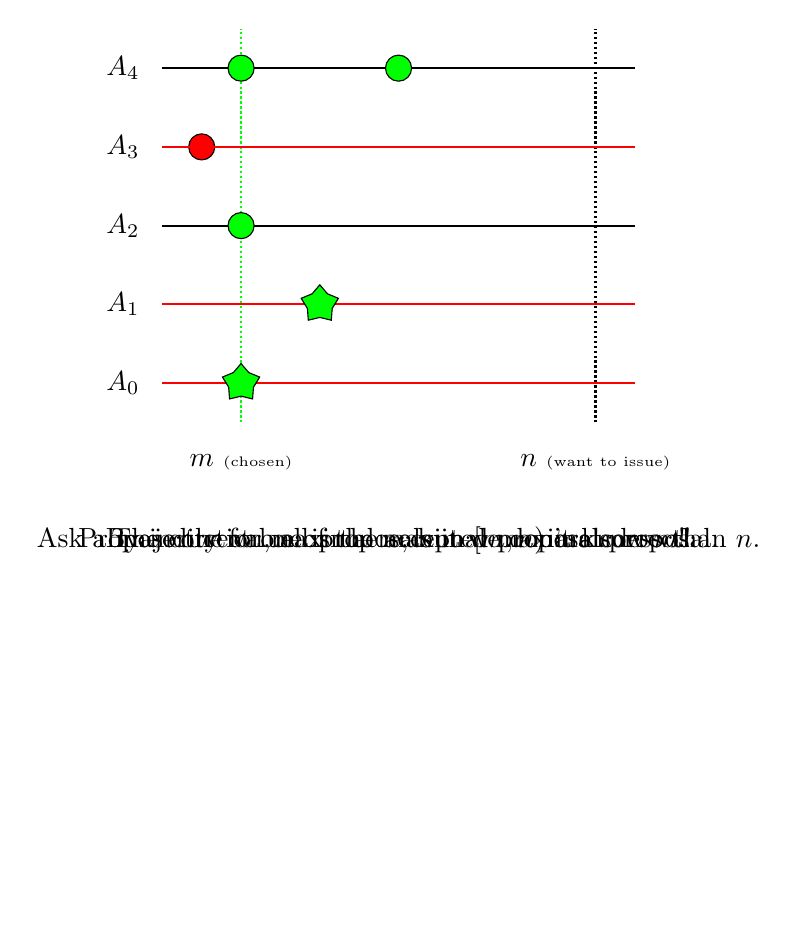
\begin{tikzpicture}
    \tikzstyle{every node} = [shape=circle]
    \foreach \n in {0, 1, 2, 3, 4} {
      \node at (-0.5, \n) {$A_\n$};
      \draw [thick] (0, \n) -- (6, \n);
    }

    \draw [thick, densely dotted, green] (1, -0.5) -- (1, 4.5);
    \node at (1, -1) {$m$ \tiny (chosen)};
    \draw [thick, densely dotted] (5.5, -0.5) -- (5.5, 4.5);
    \node at (5.5, -1) {$n$ \tiny (want to issue)};

    \node [draw, fill=red] at (0.5, 3) {};

    \foreach \n in {0, 2, 4}
      \node [draw, fill=green] at (1, \n) {};

    \node [draw, fill=green] at (2, 1) {};
    \node [draw, fill=green] at (3, 4) {};

    \visible<2->{
        \foreach \n in {0, 1, 3}
            \draw [thick, red] (0, \n) -- (6, \n);
    }
    \visible<2> {
        \node at (3, -2) { Ask a majority for maximal accepted proposals less than $n$.};
    }

    \visible<3> {
        \node [draw, star, star points=5, fill=green] at (1, 0) {};
        \node at (3, -2) { The correct one is there, but we don't know $m$! };
    }
    \visible<4-> {
        \node [draw, star, star points=5, fill=green] at (2, 1) {};
    }
    \visible<4> {
        \node at (3, -2) { By induction, all proposals in $[m, n)$ are correct! };
    }
    \visible<5> {
        \node at (3, -2) { Propose the value of the maximal maximal proposal. };
    }
  \end{tikzpicture}
  \end{figure}
\end{frame}

\begin{frame}{Maintaining $P2^b$: another picture}
  \begin{figure}[!h]
  \centering
  \begin{tikzpicture}
    \tikzstyle{every node} = [shape=circle]
    \foreach \n in {0, 1, 2, 3, 4} {
      \node at (-0.5, \n) {$A_\n$};
      \draw [thick] (0, \n) -- (6, \n);
    }

    \draw [thick, densely dotted] (5.5, -0.5) -- (5.5, 4.5);
    \node at (5.5, -1) {$n$ \tiny (want to issue)};

    \node [draw, fill=red] at (0.5, 3) {};
    \node [draw, fill=blue] at (1.5, 1) {};

    \foreach \n in {0, 2, 4}
        \draw [thick, red] (0, \n) -- (6, \n);
    \node at (3, -1.5) {If a majority has no accepted proposals, free to propose anything.};
  \end{tikzpicture}
  \end{figure}
\end{frame}

\begin{frame}{More on $P2^b$}
  \begin{itemize}
    \item Is it enough to just ask a majority of acceptors for their maximal accpted proposals and re-propose the value of the maximum one?
  \end{itemize}
\end{frame}

\begin{frame}{Not if there are many proposers!}
  \begin{figure}[!h]
  \centering
  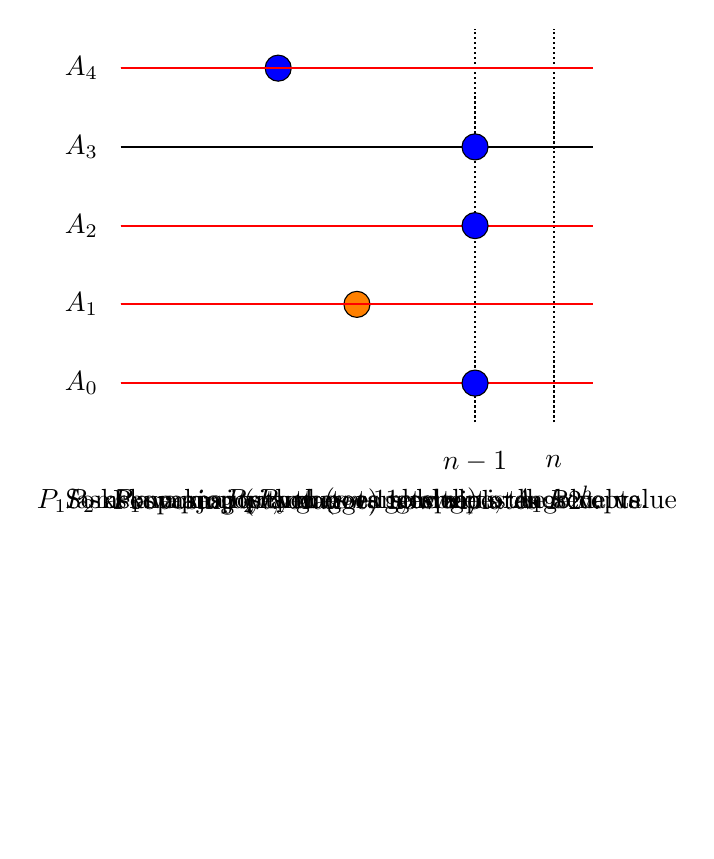
\begin{tikzpicture}
    \tikzstyle{every node} = [shape=circle]
    \foreach \n in {0, 1, 2, 3, 4} {
      \node at (-0.5, \n) {$A_\n$};
      \draw [thick] (0, \n) -- (6, \n);
    }

    \draw [thick, densely dotted] (5.5, -0.5) -- (5.5, 4.5);
    \node at (5.5, -1) {$n$};
    \draw [thick, densely dotted] (4.5, -0.5) -- (4.5, 4.5);
    \node at (4.5, -1) {$n-1$};

    %\node [draw, fill=red] at (0.5, 3) {};
    %\node [draw, fill=green] at (1.5, 2) {};
    \node [draw, fill=blue] at (2, 4) {};
    %\node [draw, fill=gray] at (2.5, 0) {};
    \visible<1,2>{
        \foreach \n in {1, 2, 4}
          \draw [thick, red] (0, \n) -- (6, \n);
    }
    \visible<1> {
        \node at (3, -1.5) {$P_1$ asks a majority wrt $n-1$ and gets the blue value};
    }
    \visible<2> {
        \node at (3, -1.5) {$P_1$ goes to sleep.};
    }

    \visible<3->{
      \node [draw, fill=orange] at (3, 1) {};
    }
    \visible<3>{
      \node at (3, -1.5) {Someone proposes the orange value, $A_1$ accepts.};
    }

    \visible<4,5>{
      \foreach \n in {0, 1, 4}
        \draw [thick, red] (0, \n) -- (6, \n);
    }
    \visible<4>{
      \node at (3, -1.5) {$P_2$ asks a majority wrt $n$, gets the orange value.};
    }
    \visible<5>{
      \node at (3, -1.5) {$P_2$ then goes to sleep.};
    }

    \visible<6->{
      \foreach \n in {0, 2, 3}
        \node [draw, fill=blue] at (4.5, \n) {};
    }
    \visible<6>{
      \node at (3, -1.5) {$P_1$ wakes up and ($n-1$, blue) is chosen.};
    }
    \visible<7>{
      \node at (3, -1.5) {Proposing ($n$, orange) now violates $P2^b$.};
    }

  \end{tikzpicture}
  \end{figure}
\end{frame}

\begin{frame}{The problem with $P2^b$}
  \begin{itemize}
    \item The problem is that to maintain $P2^b$, we need to know the maximal proposal less than $n$ that was \alert{or will ever be} accepted by some majority of acceptors.
    \item Can't predict the future -- enforce it!
    \item Make the acceptors \alert{promise} not to accept any proposal less than $n$ when responding to an initial request from a proposer.
  \end{itemize}
\end{frame}

\begin{frame}{Fixing $P1$.}
  The promises break $P1$. Let us tweak it a bit.

  \begin{invariant}[$P1^a$]
    An acceptor must accept any proposal it receives if it has not promised not to do so.
  \end{invariant}

  This is still good enough, because if there is only one proposer $P$, then no promises will be made that could impede its progress, so its proposal will be accepted.
\end{frame}

\begin{frame}{Invariants recap}
  \begin{invariant}[$P1^a$]
    An acceptor must accept any proposal it receives if it has not promised not to do so.
  \end{invariant}
  \begin{invariant}[$P2^b$]
    If a proposal with value $v$ is chosen, then every higher-numbered proposal \alert{issued} by any proposer has value $v$.
  \end{invariant}
  \begin{invariant}[P3]
    A value of the proposal is uniquely determined by its number.
  \end{invariant}
  These invariants are enough to build a safe and resilient consensus protocol.
\end{frame}

\begin{frame}{Protocol: the proposer}
  \begin{itemize}
    \item Choose a unique proposal number $n$.
    \item Send a message $\textsc{prepare}(n)$ to a majority $M$ of acceptors.
    \item Collect responses $Pr_M = \{ \textsc{promise}_m(n, n', v') \mid m \in M \}$ from $M$,  where $v'$ can be a value or $\bot$ (in which case $n' = -\infty$) if $m$ has never accepted anything.
    \item Select $v^*$ = the value of a promise with maximal $n'$ among $Pr_M$.
    \item If $v^* = \bot$, choose $v^*$ arbitrarily.
    \item Send a message $\textsc{accept}(n, v^*)$ to $M$.
  \end{itemize}
\end{frame}

\begin{frame}{Protocol: the acceptor}
  \begin{itemize}
    \item Upon receiving $\textsc{prepare}(n)$ and we have never received a $\textsc{prepare}(m)$ with $m > n$, respond with $\textsc{promise}(n, n', v')$ where $(n', v')$ is the maximal proposal numbered less than $n$ that we have ever accepted (or $(-\infty, \bot)$ if none) and record that we have promised not to accept proposals numbered less than $n$.
    \item Upon receiving $\textsc{accept}(n, v)$, accept $(n, v)$ if we have not promised not to do so.
  \end{itemize}
\end{frame}

\begin{frame}
  \begin{itemize}
  \item The protocol satisfies the invariants $P1^a, P2^b$ and $P3$, so it is a safe consensus protocol.
  \item Note that in its current form, the value is chosen by the system as a whole. No single process really learns the value yet. We'll deal with that later.
  \item Is our protocol \alert{live}?
  \end{itemize}
\end{frame}

\begin{frame}{No, even with strict synchrony assumptions.}
  \begin{figure}[!h]
  \centering
  \begin{tikzpicture}[scale=1.5]
    \tikzstyle{every node} = [shape=circle]
      \node at (-0.5, 2) {$P_1$};
      \node at (-0.5, 3) {$P_2$};
      \node at (-0.5, 0) {$\mathbb{A}$};
      \foreach \n in {2, 3} {
        \draw (0, \n) -- (3.25, \n);
        \draw [dotted] (3.25, \n) -- (6, \n);
      }
      \draw [very thick] (0, 0) -- (3.25, 0);
      \draw [dotted, very thick] (3.25, 0) -- (6, 0);

      \draw [->] (0.5, 2) -- (1, 0);
      \draw [->] (1, 0) -- (1.5, 2);
      \node at (1, -0.5) {\tiny \textsc{prepare}$(n_1)$};

      \draw [->] (1, 3) -- (1.75, 0);
      \draw [->] (1.75, 0) -- (2.5, 3);
      \node at (1, 3.25) {\tiny \textsc{prepare}$(n_1 > n_2)$};

      \draw [dashed, thick, ->, red] (1.5, 2) -- (2, 0);
      \node at (2.25, -0.5) {\tiny \textsc{accept}$(n_1, v_1)$};

      \draw [dashed, thick, ->, red] (2.5, 3) -- (3.25, 0);
      \node at (2.5, 3.25) {\tiny \textsc{accept}$(n_2, v_2)$};

      \draw [->] (2, 2) -- (2.5, 0);
      \draw [->] (2.5, 0) -- (3, 2);
      \node at (2, 2.5) {\tiny \textsc{prepare}$(n_3 > n_2)$};
  
  \end{tikzpicture}
  \end{figure}
\end{frame}

\begin{frame}{This is not a coincidence.}
  \begin{theorem}[Fischer, Lynch, Patersson '85]
    In an asynchronous system with \alert{at most one} faulty process, a consensus protocol cannot be both safe and live.
  \end{theorem}
  \begin{itemize}
    \item We'll talk about it in more detail if time permits.
    \item For our protocol to be live, it is necessary that there is only one \alert{distinguished proposer} that issues proposals. Electing one is a weak form of consensus, so some synchrony is required.
    \item Multiple proposers can only impede progress; \alert{safety is never compromised}.
  \end{itemize}
\end{frame}

\begin{frame}{Interlude: eventually synchronous systems}
  \begin{figure}[!h]
  \centering
  \begin{tikzpicture}
    \tikzstyle{every node} = [shape=circle]
    \draw [thick, ->] (0, 0) -- (5,0);
    \draw [thick, ->, green] (5, 0) -- (10, 0);
    \node at (10.1, -0.1) {$t$};
    \node [draw, fill=black] at (5, 0) {};
    \node at (5, -0.5) {\small GST};
    \node at (2.5, -0.25) {\tiny totally asynchronous};
    \node at (7.5, -0.25) {\tiny synchronous, no failures};
  \end{tikzpicture}
  \end{figure}
  \begin{itemize}
    \item Global Stabilization Time (GST) is unknown to the processes.
    \item After GST, no processes fail, no messages are lost and message delays and clock drift become bounded (but still unknown to the processes).
    \item In theory, everything remains synchronous forever. In practice, it is enough for the synchrony period to be long enough for some useful work to be done.
  \end{itemize}
\end{frame}

\begin{frame}{Synchronous leader election (an example)}
  \begin{figure}[!h]
  \centering
  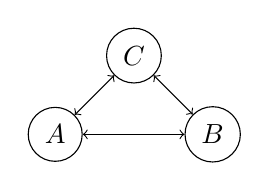
\begin{tikzpicture}
    \tikzstyle{every node} = [shape=circle]
    \node (a) [draw] at (0, 0) {$A$};
    \node (b) [draw] at (2, 0) {$B$};
    \node (c) [draw] at (1, 1) {$C$};
    \draw [<->] (a) -- (b);
    \draw [<->] (b) -- (c);
    \draw [<->] (a) -- (c);
  \end{tikzpicture}
  \end{figure}
  \begin{itemize}
    \item Everyone pings everyone else once in a while.
    \item A process considers itself the leader if it has not seen pings from processes with larger names in a while.
    \item This converges after GST.
  \end{itemize}
\end{frame}

\begin{frame}{Learning the chosen value}
  \begin{itemize}
    \item So now we have a distinguished proposer.
    \item Let's also make it a distinguished \alert{learner}!
  \end{itemize}
\end{frame}

\begin{frame}{The Paxos protocol}
  \begin{figure}[!t]
  \centering
  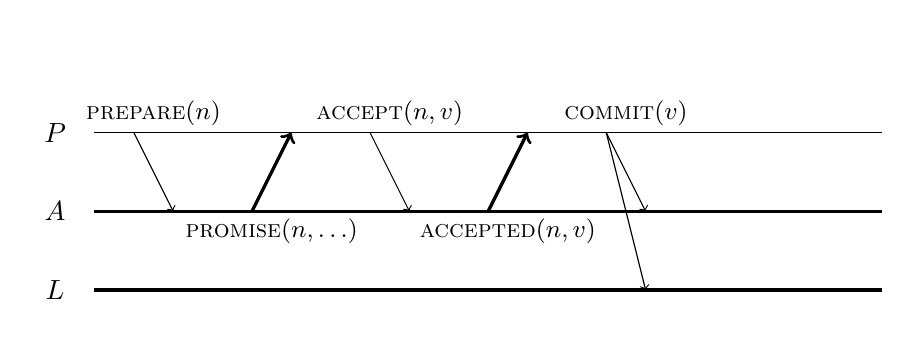
\begin{tikzpicture}
    \tikzstyle{every node} = [shape=circle]
      \node at (-0.5, 0) {$\mathbb{L}$};
      \node at (-0.5, 1) {$\mathbb{A}$};
      \node at (-0.5, 2) {$P$};

      \foreach \n in {0, 1} {
        \draw [very thick] (0, \n) -- (10, \n);
      }
      \draw (0, 2) -- (10, 2);

      \node at (0.75, 2.25) {\small \textsc{prepare}$(n)$};
      \draw [->] (0.5, 2) -- (1, 1);
      \node at (2.25, 0.75) {\small \textsc{promise}$(n, \ldots)$};
      \draw [->, very thick] (2, 1) -- (2.5, 2);
      \node at (3.75, 2.25) {\small \textsc{accept}$(n, v)$};
      \draw [->] (3.5, 2) -- (4, 1);
      \node at (5.25, 0.75) {\small \textsc{accepted}$(n, v)$};
      \draw [->, very thick] (5, 1) -- (5.5, 2);
      \node at (6.75, 2.25) {\small \textsc{commit}$(v)$};
      \draw [->] (6.5, 2) -- (7, 1);
      \draw [->] (6.5, 2) -- (7, 0);
      
  \end{tikzpicture}
  \end{figure}
  Invented by Leslie Lamport in 1989.
\end{frame}
\end{document}


